\documentclass{article}

\usepackage[margin=1in]{geometry}
\usepackage{amsmath}
\usepackage{graphicx}
\usepackage{multicol}
\usepackage{fancyvrb}

\begin{document}
	
\title{ESOF 422 - Homework 1}
\author{Nathan Stouffer and Kevin Browder}

\maketitle
\newpage

\section*{Question 1}
\subsection*{Part 1}
\begin{Verbatim}
--getCharge operation in Rental class
getCharge():Real
	begin
		declare wrkCh:Real, m:Movie, pc:PriceCode,dy:Integer;
		m:=self.getMovie();
		dy:=self.getDaysRented();
		pc:=m.getPriceCode();

		wrkCh:=0;

		if pc=PriceCode::regular then
			wrkCh:=2.0;
			if dy > 2 then
				wrkCh:=wrkCh + (dy -2) * 1.5;
			end;
		end;

		if pc=PriceCode::family then
			wrkCh:=1.5;
			if dy > 3 then
				wrkCh:=wrkCh + (dy -3) * 1.5;
			end;
		end;

		if pc=PriceCode::newRelease then
			wrkCh:=dy * 3.0;
		end;

		result:=wrkCh;
end

--getTotalCharge operation in customer class
getTotalCharge():Real
	begin
		declare totalCharge:Real, ch:Real;
		totalCharge:=0;
		for ren in self.rentals do
			ch:=ren.getCharge();
			totalCharge:=totalCharge + ch;
		end;
		result:=totalCharge;
	end;
\end{Verbatim}
\subsection*{Part 2}
\begin{figure}
	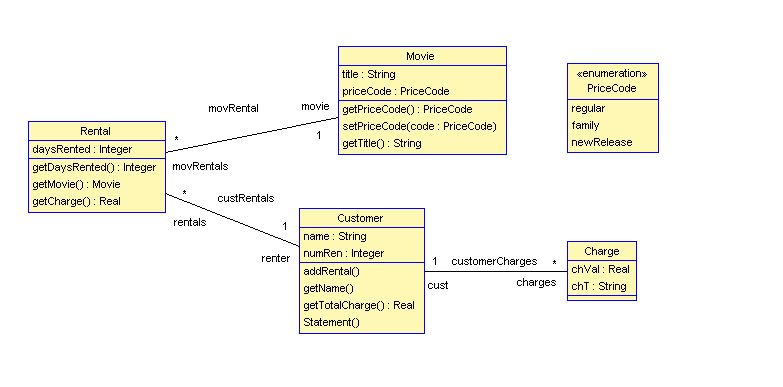
\includegraphics[width=\linewidth]{Q1Class.PNG}
	\caption{Class Diagram}
	\label{fig:class}
\end{figure}
\begin{figure}
	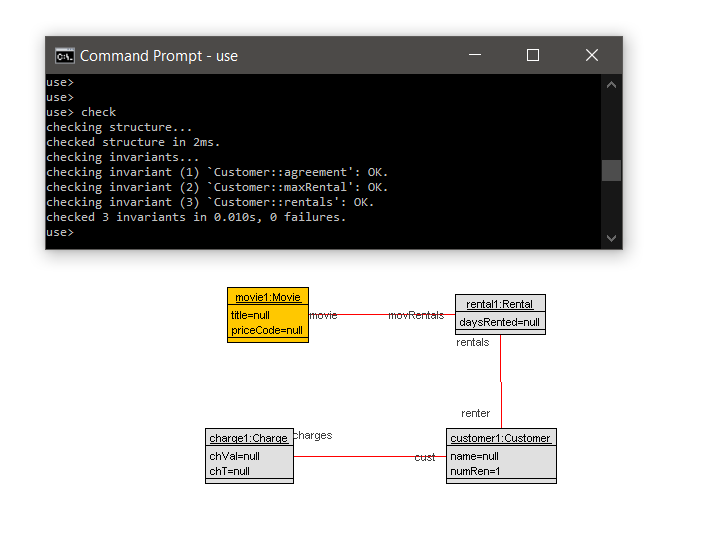
\includegraphics[width=\linewidth]{Q1ObjPNG.PNG}
	\caption{Object Diagram}
	\label{fig:obj}
\end{figure}
\begin{figure}
	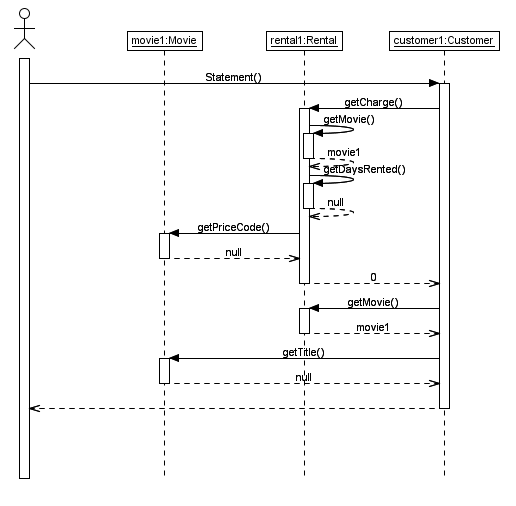
\includegraphics[width=\linewidth]{Q1Sequence.PNG}
	\caption{Sequence Diagram}
	\label{fig:seq}
\end{figure}
\section*{Question 2}
\subsection*{.x}
\begin{Verbatim}

\end{Verbatim}

\end{document}